% =====================================================================
\section{Introduction}
\label{sec:intro}
% =====================================================================

%Need for XAI on spatiotemporal data and classical Shap methods
Spatiotemporal data, such as 3D motion skeletons, multi-lead electrocardiograms, and audio signals, are used in machine learning for safety-critical domains including clinical diagnostics and monitoring. In these settings, practitioners often demand explainability alongside predictive accuracy. Beyond knowing that a prediction is accurate, they wish to understand which spatial components of a sequence, and at which times, drove that prediction.
%
Shapley-value attribution \citep{shapley1953value,lundberg2017unified} is
one of the most widely deployed tools to quantify the importance of input features in a model's final prediction
\citep{arrieta2020explainable,slack2020fooling}. For example, it quantifies which joints in a patient's skeleton drive a Parkinson's severity prediction. The method treats model inputs as \textit{players} in a cooperative \textit{game} and computes the contribution, called Shapley value, of each player to the prediction.

Computing Shapley values requires computing the model's updated prediction when it is only shown a subset of players, for many different subsets. Since standard models cannot accept missing inputs, absent features are imputed using a variety of methods. Two active lines of work adapt the classical Shapley method to structured temporal data. \emph{Manifold-aware} variants change the imputer, restricting imputed players to the data manifold
\citep{frye2021shapley,aas2021explaining,olsen2022using,taufiq2023manifold, zhang2026axiomatic}.  \emph{Temporal} variants organize the players in terms of time steps, and thus report attributions on a temporal scale~\citep{bento2021timeshap,NAYEBI2023104438,villani2022feature,
de2025shats}.
%
Each of those Shapley variants makes a series of design choices in the process of producing an explanation. The first choice defines what counts as players (whole time windows, whole joints, or fine joint$\times$window cells). The second choice defines how masked players are replaced (zeros, averages, copies of other sequences, or samples from a generative model of the data manifold). The third choice decides how the cooperative game is played, and what the ground truth, if it existed, would even be. The final choice is the \emph{metric} used to grade the quality of the explanation, with or without access to that ground truth.
%
% problem on shap for spatiotemp data
%
These design choices, while critical to the outcome, are, to the best of our knowledge, never benchmarked jointly. This is especially critical for spatiotemporal data, which exhibits both feature dependence across channels and temporal coherence. 



\begin{figure}[t]
  \centering
  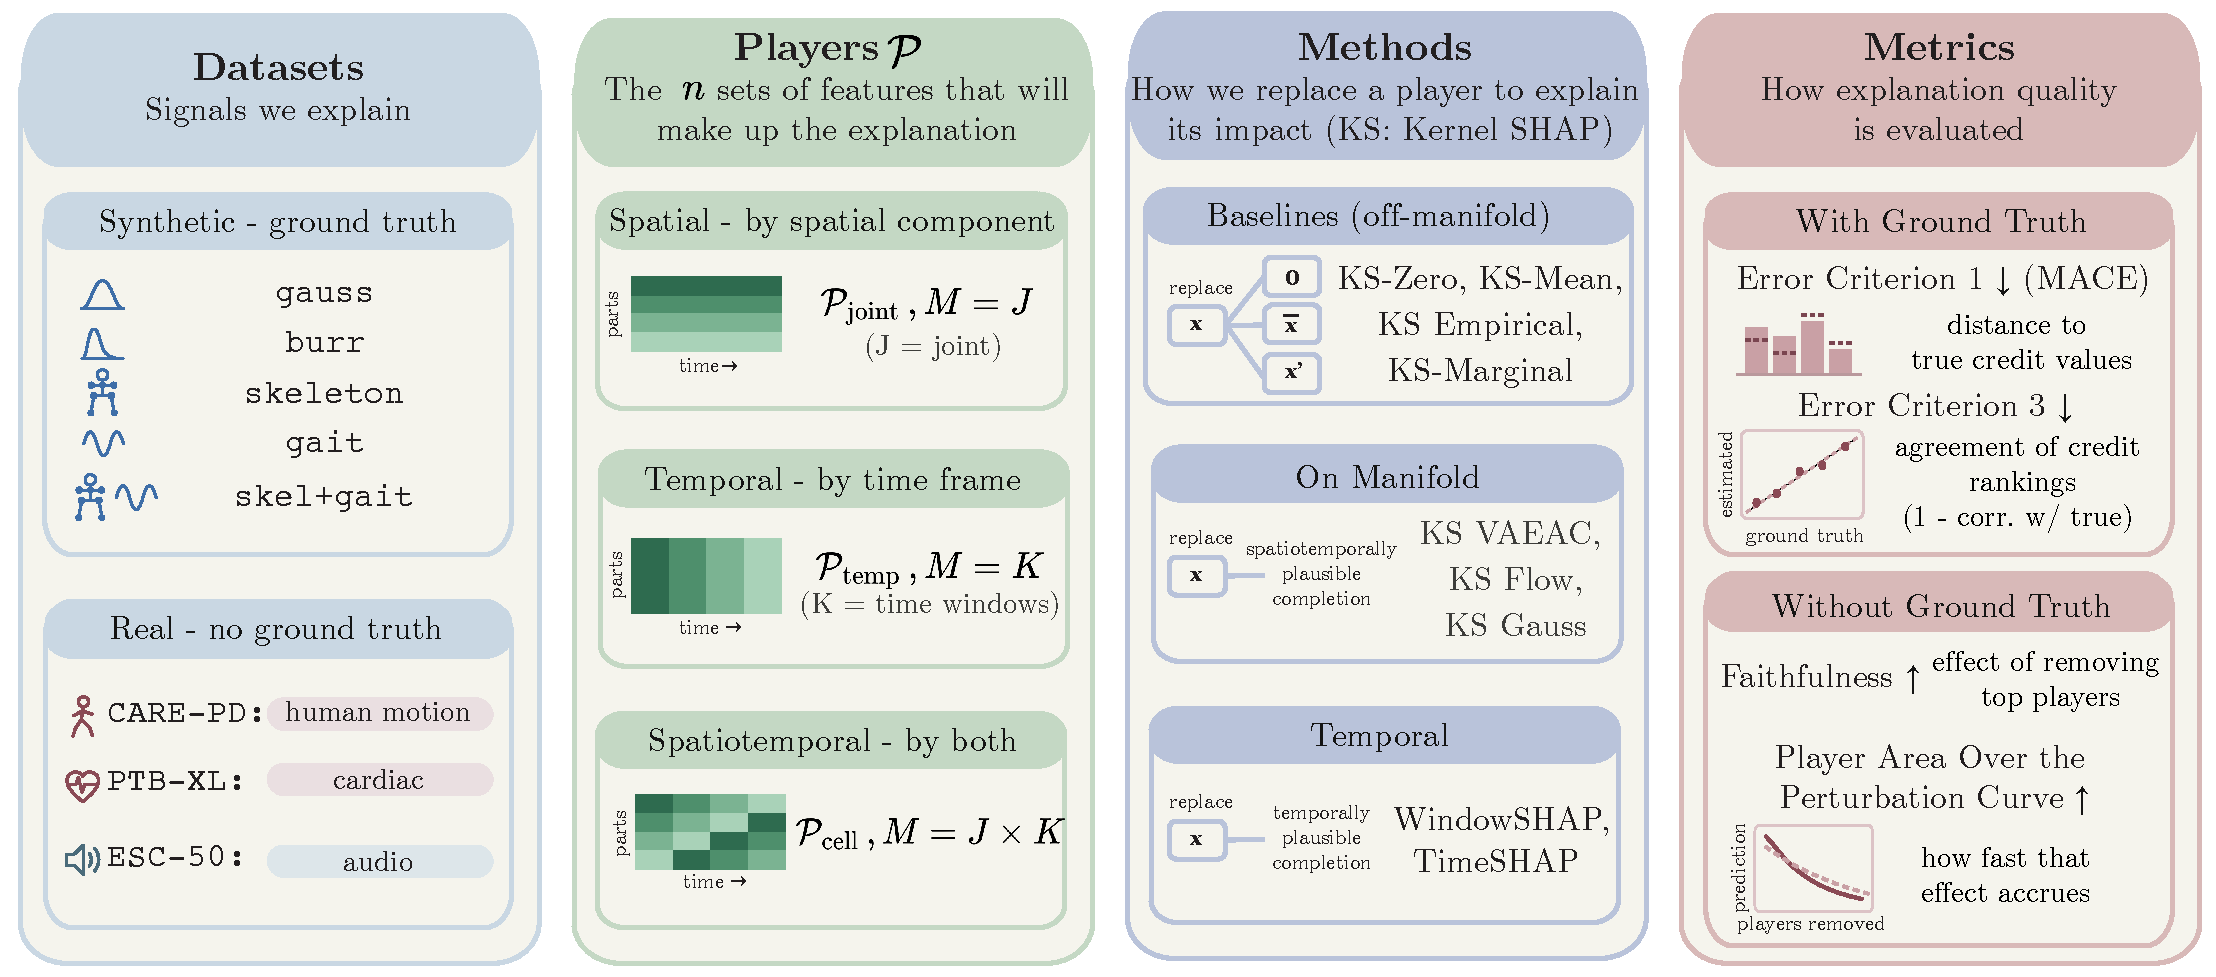
\includegraphics[width=1.0\linewidth]{figures/MotionSHAP_overview_detailed.pdf}
  % \caption{\textbf{MotionBench-XAI at a glance.}  The benchmark's axes:
  % datasets (synthetic with exact oracles, real without), player sets, SHAP
  % method families, and metrics (with and without ground truth).}
  \caption{\textbf{MotionBench-XAI} evaluates spatiotemporal Shapley value attributions as a feature-based explainability method. 
\textit{Datasets (first column):} Five synthetic spatiotemporal datasets paired with ground-truth Shapley values, and three real-world datasets. 
\textit{Players $\mathcal{P}$ (second column):} Input features partitioned spatially ($P_{\text{joint}}$), temporally ($P_{\text{temp}}$), or across a spatiotemporal grid ($P_{\text{cell}}$). 
\textit{Imputation methods (third column):} Strategies for replacing absent players via off-manifold baselines, on-manifold generative models, or temporal SHAP variants. 
\textit{Metrics (fourth column):} Evaluation via exact attribution error and linear agreement error for synthetic cases, or proxy metrics (faithfulness, PlayerAOPC) for real-world cases where ground truth is absent.}
  \label{fig:overview}
\end{figure}

 % solution on shap for spatiotemp data
\paragraph{Contributions.}
To remedy this, we propose \textbf{MotionBench-XAI}, a benchmark to compare on and off-manifold Shapley methods on data with both feature dependence and temporal coherence (Figure~\ref{fig:overview}).  In both synthetic and real-world settings, MotionBench-XAI serves as an evaluation instrument to measure how hidden design choices dictate explanation quality for spatiotemporal data.
\begin{itemize}[leftmargin=*]
\item We construct five spatiotemporal dataset families from varied distributions with closed-form marginal and conditional expectations, allowing ground-truth Shapley values  per trained classifier (\S\ref{sec:datasets-synth}, \S\ref{sec:bg-gt}).
\item We perform a systematic sweep of every combination of player set (temporal, spatial, spatiotemporal), imputation family (standard, temporal, generative), ground truth, and metric, per dataset and per classifier, using one explanation pipeline (\S\ref{sec:results-synth}).
\item We run the same pipeline on three real datasets where
  ground truth is not available (\S\ref{sec:datasets-real}): clinical gait (CARE-PD;
  \citealp{adeli2025multi}), 12-lead ECG (PTB-XL;
  \citealp{wagner2020ptbxl}), and environmental audio (ESC-50;
  \citealp{piczak2015esc}) (\S\ref{sec:results-real}).
\item We summarize findings with direct practical consequence for practitioners using Shapley explanations in applied settings, distilled into a practical guide (Fig. \ref{fig:decision}).
\end{itemize}

\S\ref{sec:related} situates MotionBench-XAI within the literature detailing how it resolves current evaluation gaps. All code and  checkpoints are released at \href{https://anonymous.4open.science/r/motionbench-xai-41C7}{anonymous.4open.science/r/motionbench-xai-41C7} (Appendix~\ref{app:repro}).
